\section{Desarrollo}

\subsection{Diseño}

Con el diseño implementado los dos botones al presionarse van a conectar el pin D2 a +5V, y  la corriente máxima que estos pines pueden proporcionar es de 40 mA. Sin embargo para asegurar el funcionamiento se limitó la corriente a 30 mA.

El valor de la tensión de los LEDs es de 2.0 V. Por lo tanto, utilizando Ley de Kirchhoff para calcular el valor de las resistencias para el caso de un solo LED:

\begin{equation}
    R = \frac{V_{DD} - V_{LED}}{I_{Max}} = \frac{5 - 2.0}{25 mA} =  120\Omega
\end{equation}

Tomando los valores en bodega de la escuela, se eligieron entonces resistencias de para cada uno de los LEDs de $120 \Omega$. Estas resistencias son de gran importancia para proteger los LEDs.

Además, es de suma importancia notar que un circuito RC se agregó para proteger de los efectos rebote a los botones. Se definió una resistencia de $10 K\Omega$ debido a que proporciona una corriente limitada a través del circuito para reducir el consumo de energía y la carga en la fuente de alimentación, seguidamente el capacitor de 10 nF ofrece un buen equilibrio entre filtrado y velocidad de respuesta de los botones. \cite{drmaker2014debouncing}

El tiempo que transcurre desde que se presiona el pulsador momentáneo hasta que el condensador se carga por completo se puede calcular utilizando la siguiente fórmula:

\begin{equation}
    Tiempo (segundos) = {Valor de R} \cdot {Capacidad del condensador}
\end{equation}

Calculando con los valores que se diseñaron para el circuito:

\begin{equation}
    Tiempo (segundos) = 10 K\Omega \cdot 10 nF
\end{equation}

\begin{equation}
    Tiempo (segundos) = 10 K\Omega \cdot 10 nF
\end{equation}

\begin{equation}
    Tiempo (segundos) = 0.1 s
\end{equation}

Este tiempo permite una respuesta lo suficientemente rápida para que el semáforo peatonal se active después de que el usuario presione el botón, y al mismo tiempo elimina de manera efectiva cualquier rebote en el interruptor

A nivel del código implementado, se puede mencionar que se agregaron ciertas características para poder optimizar el rendimiento y código. Entre ellas destacan el uso de macros para definir valores constantes y representar unidades de tiempo clave.

El uso de macros permiten asignar nombres significativos a valores numéricos, lo que hace que el código sea más legible, reutilizable y fácil de mantener. Además, las macros facilitan la modificación de estos valores en un solo lugar, lo que simplifica la adaptación del comportamiento del semáforo sin necesidad de buscar y cambiar cada instancia numérica en el código. Esta característica puede mejorar la escalabilidad del código, ya que cualquier ajuste necesario en los tiempos de cambio de estado o ciclos del temporizador se puede realizar de manera eficiente y precisa simplemente modificando las macros. 

Además otra implementación importante fue el uso de funciones \textit{inline} para funcionalidades como el parpadeo de las luces del semáforo y la gestión de las interrupciones.  ERste tipo de funciones se utilizan para evitar la sobrecarga de llamadas a funciones y, en su lugar, insertar directamente el código de la función en el lugar donde se invoca. Esto ahorra el tiempo y los recursos que normalmente se consumirían en la llamada y retorno de una función, lo que resulta en un código más rápido y eficiente en términos de rendimiento. \cite{microsoftInlineFunctions}

A continuación se muestran los costos de los componentes utilizados:

\begin{table}[h]
\centering
\begin{tabular}{|c|c|}
\hline
\textbf{Componente}     & \textbf{Precio} \\ \hline
ATtiny4313               & 583 colones    \\ \hline
Resistencia de 120 Ohms & 155 colones     \\ \hline
Botón                   & 150 colones     \\ \hline
Resistencia de 10 KOhms & 120 colones     \\ \hline
10 nF capacitor        & 325 colones     \\ \hline
LED Verde              & 310 colones     \\ \hline
LED Rojo              & 310 colones     \\ \hline
\end{tabular}
\caption{Precio de los componentes}
\label{tab:componentes}
\end{table}

\newpage
\subsection{Funcionalidad del diseño}
El circuito en el simulador se muestra de la siguiente manera:
\begin{figure}[H]
    \centering
    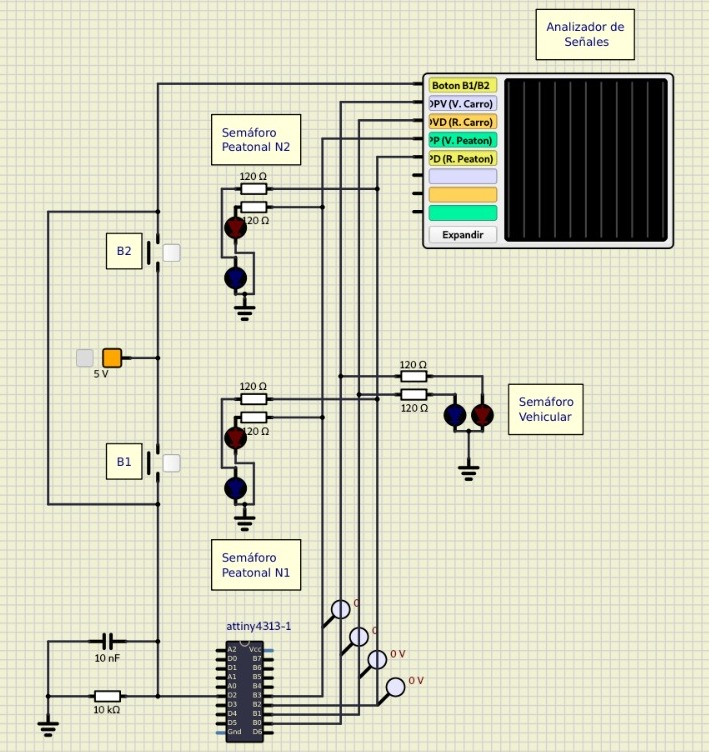
\includegraphics[scale=0.4]{images/Circuito_semaforo.jpeg}
    \caption{Diseño del circuito.}
    \label{fig:semaforo}
\end{figure}

Al poner a funcionar el simulador, se puede observar el estado inicial del semáforo a continuación. Puede notarse que en su estado inicial los semáforos peatonales se encuentran en rojo mientras que el semáforo vehicular en verse

\begin{figure}[H]
    \centering
    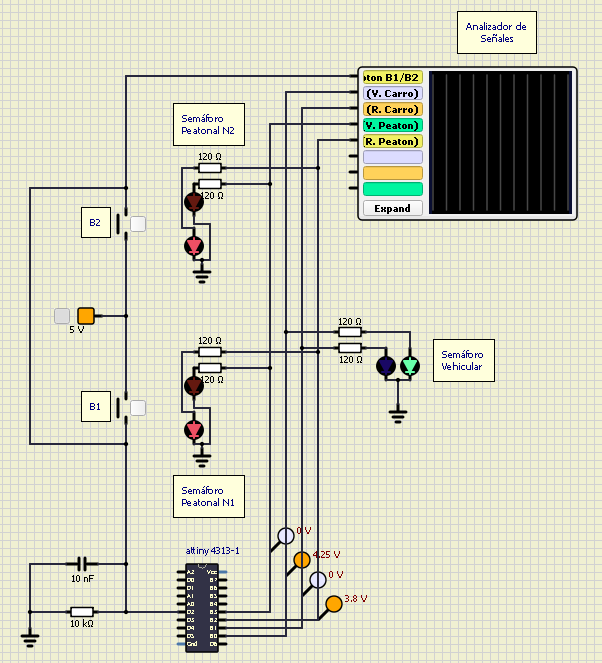
\includegraphics[scale=0.6]{images/uso1.png}
    \caption{Estado inicial del semáforo}
    \label{fig:semaforo2}
\end{figure}

Seguidamente, al presionar cualquiera de los dos botones se puede observar el semáforo peatonal en funcionamiento. El semáforo vehicular pasa a rojo mientras que los peatonales a verde


\begin{figure}[H]
    \centering
    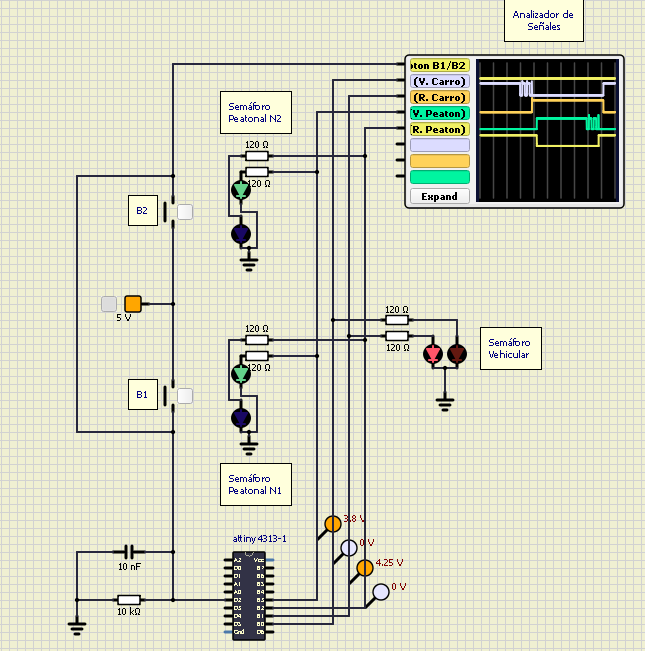
\includegraphics[scale=0.6]{images/uso2.png}
    \caption{Semáforos en funcionamiento}
    \label{fig:semaforo2}
\end{figure}

Finalmente, luego del tiempo definido para el funcionamiento de los semáforos peatonales, éstos vuelven a su estado inicial y el semáforo vehicular vuelve a estar en verde.

\begin{figure}[H]
    \centering
    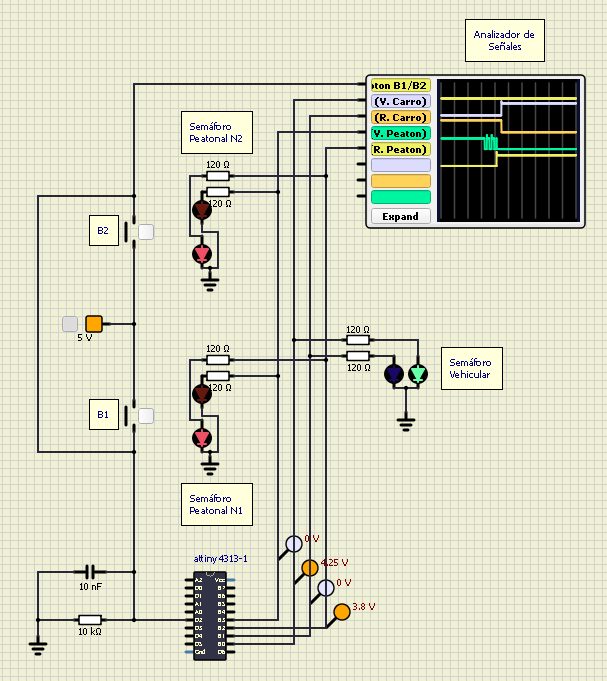
\includegraphics[scale=0.6]{images/uso3.png}
    \caption{Semáforos en funcionamiento}
    \label{fig:semaforo2}
\end{figure}

\newpage

\subsection{Diagrama de estados}
A continuación se presenta el diagrama de estados del proyecto:
\begin{figure}[H]
    \centering
    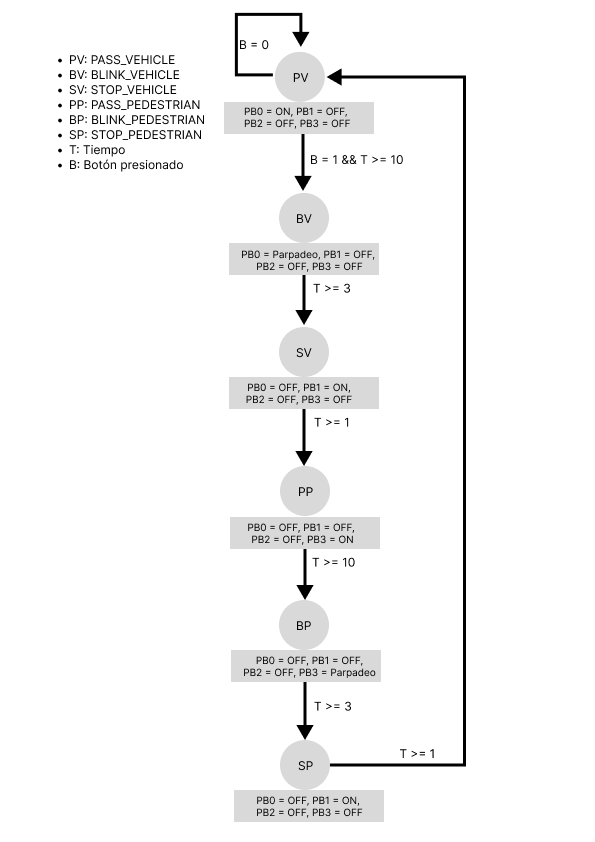
\includegraphics[scale=0.5]{images/Maquina de estados.png}
    \caption{Diagrama de estados.}
    \label{fig:diagrama_estados}
\end{figure}

\newpage
\subsection{Funcionalidad electrónica}
Se colocó un osciloscopio en las salidas de cada pin y en la entrada del botón para mostrar que los cambios en la tensión son los esperados. En la siguiente imagen se puede observar la lectura del osciloscopio.
\begin{figure}[H]
    \centering
    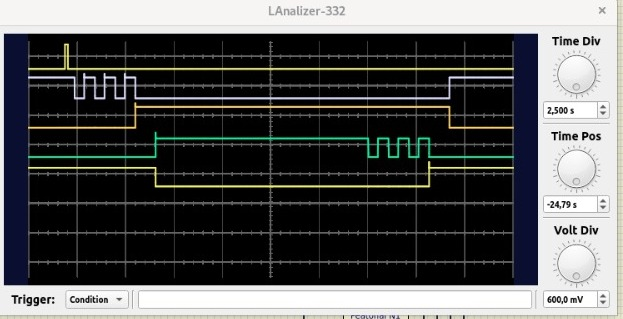
\includegraphics[scale=0.5]{images/Ondas_tiempo.jpeg}
    \caption{Lectura del osciloscopio.}
    \label{fig:diagrama_tiempo}
\end{figure}
Al inicio de las pruebas, todas las salidas se encontraban en un estado lógico bajo (`0'), cumpliendo con las expectativas iniciales. Del mismo modo, el botón de entrada también comenzó en un estado bajo. Cuando se presionó el botón, la señal asociada mostró un flanco ascendente, que activó una transición en la máquina de estados. Durante el experimento, las transiciones entre diferentes estados de las salidas se llevaron a cabo de manera coherente con la definición de la máquina de estados.

Además, se pudo verificar que cada estado se mantenía durante el período de tiempo especificado antes de avanzar al siguiente estado. Es importante destacar que durante las pruebas no se detectaron falsas transiciones ni ruido eléctrico que pudieran afectar la secuencia de estados. Esto indica que el sistema de ``debouncing'' para el botón funciona correctamente, y que la implementación de la máquina de estados funciona de la manera esperada.